\subsubsection{Merging and splitting clusters}

{\color{red}
Habría que hablar sobre implementación (Copio y pego de lo que ya tenía escrito en español... escribo algo parecido pero en inglés??)\\

En el contexto de la robótica, resulta muy pertinente discutir sobre diversos aspectos relacionados con la implementación. Es por ello que en esta sección introduciremos tres posibles estrategias para poner en práctica nuestro algoritmo de búsqueda sobre una flota de robots.\\

Contando con un único enjambre, en una primera aproximación se puede considerar un grafo tipo estrella, donde uno de los $N$ agentes es la unidad de cómputo encargada de aproximar $L_\sigma$. Para estimar esta dirección de ascenso se hará uso de la información de cada agente $i$ con respecto a la posición $x_i$ y el valor del campo escapar $\sigma(r_i)$. Variables que deberán de ser medidas por el agente en cuestión y enviadas únicamente a la unidad de cómputo. Finalmente, la estimación de la dirección de ascenso sería compartida con todos los agentes. Siguiendo esta metodología, mientras todos los integrantes del enjambre compartan un mismo eje de referencia absoluto, se podría llevar a cabo una implementación que preserve las garantías del algoritmo.

El principal problema del grafo tipo estrella que es que toda la coordinación depende de un único agente, lo que la hace poco robusta. Si la unidad de cómputo desaparece, el enjambre debería de seleccionar si es posible a otro líder para poder continuar con la misión. Una solución inmediata a este problema es considerar un grafo completo, donde la toda información recogida debería de ser compartida con todos los integrantes del enjambre. De este modo, cada agente $i$ realizaría su propia estimación de $L_\sigma$. Finalmente se compartirían todas las estimaciones $\hat L_{\sigma_i}$ realizadas para consensuar entre todos los agentes el seguimiento de una misma dirección de ascenso, que por ejemplo podría ser $\hat L_{\sigma} = \frac{1}{N}\sum_{i=1}^N\hat L_{\sigma_i}$.

Con el objetivo de relajar la exigencia en términos de cálculo y comunicaciones que propone el caso del grafo completo, propondremos una estrategia intermedia. Se desplegará un número $N_c$ de enjambres. Cada uno de ellos contará con $N_k$ agentes, formando una geometría con respecto a su centroide $^kr_c$ que denotaremos con el vector $X_k = (^kx_{1}^T, \dots, {}^kx_{N_k}^T)^T$, donde $^kx_i$ es la posición del agente $i$ con respecto al centroide del grupo $k$. A todos los enjambres se les asignará la misión de buscar la fuente $r^*$ del campo escalar $\sigma(r)$. De este modo, la unidad de cómputo de cada grupo se encargará de aproximar desde su centroide una dirección de ascenso
}

\newpage

\begin{figure}[!h]
    \centering
    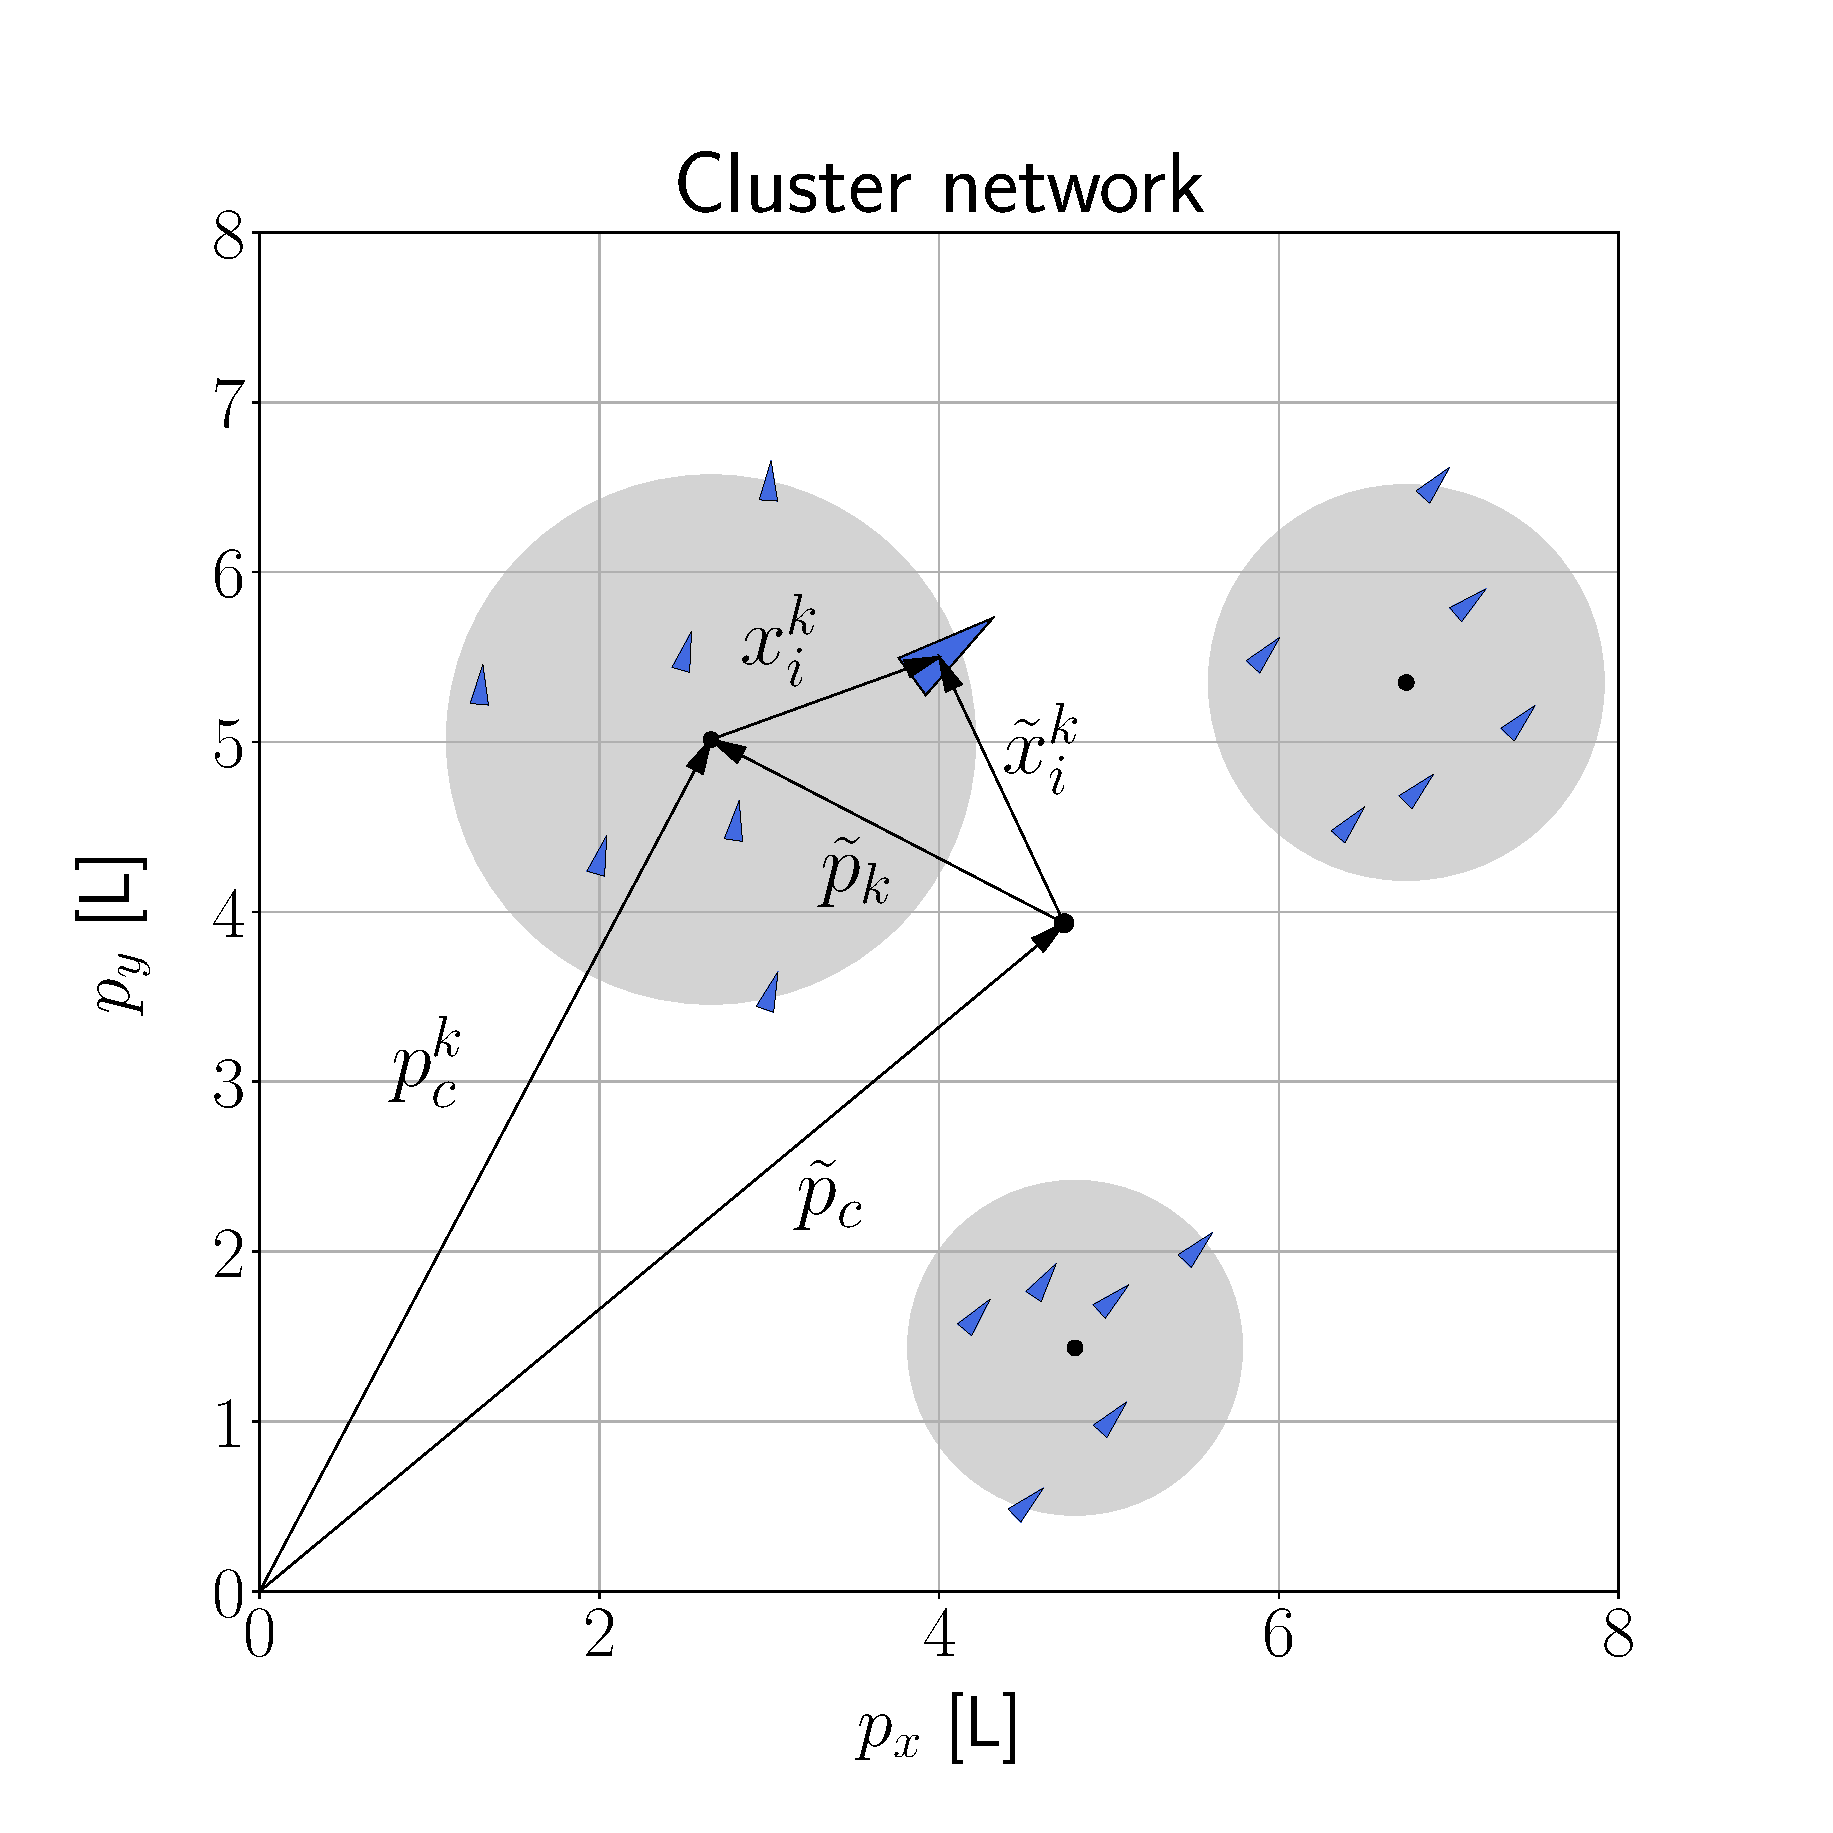
\includegraphics[trim={0 0 0 1.0cm}, clip, width=0.6\columnwidth]{./fig/pctilde.eps}
    \caption{A robot cluster $k$ with centroid at $p_c^k$ described by $\Tilde p_c$, the centroid of the cluster network.}
    \label{fig: pctilde}
\end{figure}

% With -> Given
Given $\Tilde p_c := \frac{1}{N_c}\sum_{k=1}^{N_c}p_c^k$ as the centroid of the cluster network, we propose the following vector as a possible ascending direction at $\Tilde p_c$:

\begin{equation} \label{eq: L_tilde}
    \Tilde{L} = \frac{1}{N_c}\sum^{N_c}_{k=1}L_k(p_c^k, x_i^k)
\end{equation}

Here

\begin{equation}
    L_k = \frac{1}{N_k D_k^2}\sum^{N_k}_{i=1}\sigma(p_c^k + x_i^k)x_i^k = \frac{1}{N_k D_k^2}\sum^{N_k}_{i=1}\sigma(\Tilde p_c + \Tilde{x_i}^k)(\Tilde{x_i}^k - \Tilde p_c^k)
\end{equation}
 
is the $L_\sigma$ computed by each cluster, where $N_k$ represent the number of agents of cluster $k$ and $D_k = \operatorname{max}_{1\leq i\leq N_k}{||x_i^k||}$.

In order to approximate $\sigma(p)$, we apply the Taylor expansion around the point $\Tilde p_c$. This way, focusing on the $L_k$ of one cluster we can say that

\begin{align}\label{eq: l_k}
L_k & \propto \sum^{N_k}_{i=1} \left[ \sigma(\Tilde p_c) + \nabla\sigma(\Tilde p_c)^T\Tilde{x_i}^k + O\left(||\Tilde{x_i}^k||^2\right)\right] 
      (\Tilde{x_i}^k - \Tilde p_c^k) \nonumber\\
    & = \sum^{N_k}_{i=1} \left[\nabla\sigma(\Tilde p_c)^T\Tilde{x_i}^k + O\left(||\Tilde{x_i}^k||^2\right)\right] 
      (\Tilde{x_i}^k - \Tilde p_c^k).
\end{align}
\newpage

Inspired by $L_\sigma^1$, we define $\Tilde{E}_k := L_k - \Tilde{L}^1_k$ and inquire whether if the following expression is also an ascending direction:

\begin{equation}\label{eq: l1_tilde}
   \Tilde{L}_k^1 = \frac{1}{N_k D_k^2}\sum^{N_k}_{i=1} \left[ \nabla\sigma(\Tilde p_c)^T\Tilde{x_i}^k \right]
                                                       (\Tilde{x_i}^k - \Tilde p_c^k).
\end{equation}

To reply this question, let us examine the projection of $\nabla\sigma(\Tilde p_c)$ over $\Tilde{L}_k^1$:

\begin{align*}
\nabla\sigma(\Tilde p_c)^T \Tilde{L}_k^1 & = \frac{1}{N_k D_k^2} \sum^{N_k}_{i=1} 
    \left[ 
    ||\nabla\sigma(\Tilde p_c)^T\Tilde{x_i}^k||^2 
    - \left(\nabla\sigma(\Tilde p_c)^T\Tilde{x_i}^k\right) \left(\nabla\sigma(\Tilde p_c)^T\Tilde p_c^k\right) 
    \right].
\end{align*}

This expression comprises two different terms. The first one is always positive, whereas the second term is dependent on the distribution of agents and the position of the cluster $k$ observed from $\Tilde p_c$. To focus the analysis around $\Tilde p_c$, we will restrict ourselves to $\Tilde{\mathcal{S}}$, a compact set of $\mathbb{R}^m$ that includes all points within the ball of radius $\Tilde{D} = \operatorname{max}_{1\leq k\leq N_c}{(d_k + D_k)}$ centered at $\Tilde p_c$, where $d_k = ||\Tilde p_c^k||$. With this, we obtain

\begin{equation}\label{eq: l1_tilde_proj}
   \nabla\sigma(\Tilde p_c)^T \Tilde{L}_k^1 \geq 
        F_{\Tilde{\mathcal{S}}} (x_k) - K_{\Tilde{\mathcal{S}}}^2 \frac{d_k}{D_k} \frac{(d_k + D_k)}{D_k}.
\end{equation}

Thus, we can conclude that $\Tilde{L}_k^1$ is an ascending direction for a particular configuration $(x_k, d_k, D_k)$ if (\ref{eq: l1_tilde_proj}) is greater than 0. At this point, our ultimate goal is to analyze whether $\Tilde{L}_k^1$ provides a good approximation of $L_k$. To this end, we introduce the following result.

{\color{red} Generalization of Lemma 2???}
\begin{lemma}
\label{lem: l1_approx}
    For a signal $\sigma$ approximated in $\Tilde p_c$, a conservative divergence between $\Tilde{L}_k^1$ and $L_k$ {\color{red} depends linearly on $D_k$ and quadratic on $d_k$ if $d_k$ and $D_k$ are respectively fixed}, i.e.,
    $$
    ||L_k- \Tilde{L}_k^1|| \leq M \frac{(d_k + D_k)^2}{D_k}.
    $$
\end{lemma}
\begin{proof}
    From (\ref{eq: stay}), (\ref{eq: l_k}) and (\ref{eq: l1_tilde}), then it is straightforward to see that
    \begin{align*}
    ||L_k- \Tilde{L}_k^1||
        & = \frac{1}{N_k D_k^2} \sum^{N_k}_{i=1} || \left[\sigma_i - \sigma(\Tilde p_c) -  \nabla\sigma(\Tilde p_c)^T\Tilde{x}_i^k \right] x_i^k || \\
        &  \leq \frac{1}{N_k D_k^2} \sum^{N_k}_{i=1} M ||\Tilde{x_i}^k||^2 ||x_i^k||
           \leq M \frac{(d_k + D_k)^2}{D_k}.
    \end{align*}
\end{proof}

Lemma \ref{lem: l1_approx} show us how fast $\Tilde{L}^1_k$ diverges from $L_k$ in the whole space. However, if we restrict ourselves again to the compact set $\Tilde{\mathcal{S}}$, we can say that

\begin{equation}
        ||L_k- \Tilde{L}_k^1|| \leq M_{\Tilde{\mathcal{S}}} \frac{(d_k + D_k)^2}{D_k}
\end{equation}

\newpage
Since $\Tilde{E}_k = L_k - \Tilde{L}^1_k$, then we have that

\begin{align}\label{eq: E_tilde}
    \nabla\sigma(\Tilde p_c)^T \Tilde{E}_k & = \frac{1}{N_k D_k^2} \sum^{N_k}_{i=1}
        (\left[\sigma_i - \sigma(\Tilde p_c) -  \nabla\sigma(\Tilde p_c)^T\Tilde{x}_i^k \right] 
        \nabla\sigma(\Tilde p_c)^T x_i^k) \nonumber \\
        & \leq \frac{1}{N_k D_k^2} \sum^{N_k}_{i=1} M_{\Tilde{\mathcal{S}}} ||\Tilde{x_i}^k||^2 ||x_i^k||
        \leq K_{\Tilde{\mathcal{S}}} M_{\Tilde{\mathcal{S}}} \frac{(d_k + D_k)^2}{D_k}
\end{align}

Finally, if we combine (\ref{eq: l1_tilde_proj}) and (\ref{eq: E_tilde}) then we obtain the following conclusion:

\begin{align*}
   \nabla\sigma(\Tilde p_c)^T \Tilde{L}_k 
        & = \nabla\sigma(\Tilde p_c)^T \Tilde{L}^1_k + \nabla\sigma(\Tilde p_c)^T \Tilde{E}_k  \\
        & \geq F_{\Tilde{\mathcal{S}}} (x_k) 
        - K_{\Tilde{\mathcal{S}}} \frac{d_k}{D_k} \frac{(d_k + D_k)}{D_k} 
        - K_{\Tilde{\mathcal{S}}} M_{\Tilde{\mathcal{S}}} \frac{(d_k + D_k)^2}{D_k}.
\end{align*}

Thus, we can introduce a new sufficient condition to say that $L_k$ is an ascending direction:

\begin{equation}\label{eq: l_tilde_cond}
        F_{\Tilde{\mathcal{S}}} (x_k) 
        - K_{\Tilde{\mathcal{S}}} \frac{d_k}{D_k} \frac{(d_k + D_k)}{D_k} 
        - K_{\Tilde{\mathcal{S}}} M_{\Tilde{\mathcal{S}}} \frac{(d_k + D_k)^2}{D_k} > 0.
\end{equation}

% approaches - it extends the condition - ensure - holds - we can conclude
Let us note that when $d_k$ approaches zero then (\ref{eq: l_tilde_cond}) becomes similar to (\ref{eq: xiD}). This outcome is significant because it extends the condition (\ref{eq: xiD}). As a result, now we are able to approximate $\sigma(p)$ around any $p$ and determine whether $L_k$ (or $L_\sigma$) is an ascending direction in $\Tilde{\mathcal{S}}$. Therefore, focusing on (\ref{eq: L_tilde}), if we can ensure that the condition (\ref{eq: l_tilde_cond}) holds for the worst case of $\nabla\sigma(\Tilde p_c)^T \Tilde{L}_k$, then we can conclude that $\Tilde{L}$ is an ascending direction, as $\nabla\sigma(\Tilde p_c)^T \Tilde{L} > 0$.

{\color{red} (??) is (Paper 11)}

It is also interesting to highlight that {\color{red} ... (Héctor, it would be potentially illustrative if we talk here about $d_k$ and $D_k$ dependencies. However, I would like to discuss with you how to FORMALLY tell that history.)}

{\color{red} Something more to conclude???} 






